\documentclass{article}

% PREAMBLE %
\usepackage{graphicx} % for importing images
\usepackage{xcolor} %for coloring text
\usepackage{subcaption} %for subfigures
\usepackage{amsmath,amssymb,bm}
\usepackage{tikz}
\usepackage{pgfplots}
\pgfplotsset{compat=1.18}

%tikz libaries
\usetikzlibrary{calc,angles,quotes}
\usetikzlibrary{intersections} %for intersections between \paths

% CUSTOM COMMANDS %

% Bold vectors for Latin and Greek:
\newcommand{\vect}[1]{\bm{#1}}    % \vect{x}, \vect{\alpha}, \vect{\nabla}
\newcommand{\uvect}[1]{\hat{\bm{#1}}} % unit vectors: \uvect{n}

% METADATA %
\author{Thomas Dizon}
\title{CPU Graphics Engine}

% CONTENT %
\begin{document}

\maketitle

\begin{figure}[h]
	\centering
	\includegraphics[width=0.6\textwidth]{scene.png}
	\caption{}
\end{figure}

\newpage

\tableofcontents

\newpage

\section{Introduction}

\subsection{Motivation}
\begin{itemize}
\item As someone interested in developing 3D games and graphics, I was frustrated with how much I didn't understand when I used game engines like Unity and Godot. When I wanted to achieve a simple effect like adding grass, water or natural-looking terrain, I was overwhelmed with my own inability. Thus, I committed myself to building a 3D engine from scratch so I could allow these concepts that I didn't understand emerge naturally as byproducts as I worked towards the goal of rendering 3D objects. 
\item Now that I've more or less finished the project, it is A LOT easier now to imagine how to achieve some graphical effect like a grass or water shader. Since I understand how it works conceptually under the hood, the programming is a lot easier.
\item It's also a great precursor to understanding more in depth how the GPU works.
\end{itemize}

\subsection{What is a \textit{Graphics Engine}?}
\begin{itemize}
\item The 'rasterization' step in the graphics render pipline is a specific part which involves converting Primitives into Fragments
\item A primitive, in my case, is a Triangle and a Fragment is an (x,y) value on the screen with an additional z value to track its depth
\item In the real world, rasterization is done purely through specialized hardware on the GPU (which is why it is so fast)
\item To conceptually understand how it works, instead of building a GPU from scratch (hard), I'll use my good old CPU to do the rasterizing (still hard but easier)
	\item Just to clarify between similar terms. A "Software Rasterizer" refers to writing a CPU implementation of the Rasterization step in a "Software Renderer". A "Software Renderer" is a CPU implementaion of the Graphics Pipeline. A "Graphics Engine" is a CPU implementation of the graphics pipeline as well as Scene Management, Asset Management, Input handling, Updating the Scene etc. It falls short of being a fully fledged game engine but the scope is larger than a Software Renderer
\end{itemize}

\subsection{Why \textit{C}?}
\begin{itemize}
\item I first touched C during my Systems Programming course at University. It was extrememly difficult for me at the time but very benefiical for my programming skills. I felt that I haven't extracted all that I can from the language yet.
\item Also, I wanted to get as low level as possible for this project to ensure I had minimal dependencies. To truly understand the Graphics Pipeline, I wanted to build it truly (well, mostly) from scratch
\end{itemize}

\subsection{What does the project depend on?}
\begin{itemize}
\item Right now, it depends on the C standard library, std\_image.h (reference) for dealing with .png files and SDL2 (reference) for handling all the OS level stuff like inputs and writing to the screen. Though you could easily replace SDL with any other library which creates Windows for you like RayLib.
\end{itemize}

\section{The Graphics Engine}
\subsection{Diagram}
\subsection{Overview}
\begin{itemize}
\item{Preparing Assets for the Scene}
\item{Preparing the Scene}
\item{Updating the Scene}
\item{Primitive Assembly}
\item{Vertex Shader}
\item{Clipping \& Viewport}
\item{Rasterization}
\item{Fragment Shader}
\item{Output Merging \& Depth Test}
\end{itemize}

\section{3D Geometry in Memory}

\subsection{How do you represent a 3D object on a computer?}
\subsection{Vertices and Triangles}
\begin{itemize}
\item Using a Mesh
\end{itemize}
\subsection{3D Mesh}
\subsection{3D File types}

\section{Coordinate Spaces}
\subsection{What is a \textit{Coordinate Space}?}
\subsection{GameObjects \& Object Space}
\subsection{Scenes \& World Space}
\subsection{Cameras \& View Space}

\section{Transforming Vertices}
\subsection{Matrices as Transformations}

\subsection{Deriving the Model Matrix}
\subsubsection{Transforms}
\subsubsection{Scale Matrix}
\subsubsection{Rotation Matrix}
\subsubsection{Translation Matrix}
\subsubsection{Combining them together}

\subsection{Deriving the View Matrix}
\subsubsection{The Matrix Inverse}
\subsubsection{Inverse of the Model Matrix}

\subsection{The Vertex Shader}
\subsection{Perspective Projection}
\begin{itemize}
\item In a sentence, the goal of the Perspective Projection is to map the View Space 'View Frustum' to 'Canonical View Volume' in such a way that perspective is simulated.

\item The Canonical View Volume is all points (x,y,z) such that $x \in [-1,1]$, $y \in [-1,1]$ and $z \in [0,1]$ which matches the \textit{Vulkan} convention and a format understood by our rasterizer.

\item Perspective Projection is broken up into two steps:
\begin{enumerate}
\item Projection Matrix
\item Perspective Divide
\end{enumerate}

\item The \textit{Projection Matrix} transforms a vertex from View Space into Clip Space and the \textit{Perspective Divide}, which is ultimately responsible for simulating perspective, is given by the following operation: 
\[
	\begin{pmatrix}
		x\\
		y\\
		z\\
		w
	\end{pmatrix}
	\rightarrow
	\begin{pmatrix}
		x/w\\
		y/w\\
		z/w\\
		1
	\end{pmatrix}
\]

\item If you are confused, please keep reading! I go into more detail here.
\end{itemize}
\subsubsection{What is \textit{Perspective}?}
\begin{itemize}
	\item In this project, my goal is to create graphics that are visually realistic or at least somewhat consistent with our experiences in the real world. Thus, my definition of Perspective will be made with that in mind.
	\item We start by assuming the viewer is 'point like'. We, as humans, perceive the world through our eyes which are 'point-like', in contrast to something like a Photosensor which perceives the world through a rectangular array of sensors.
	\item Put simply, Perspective is the phenomenon of objects appearing smaller to a point-like viewer as it moves further away from the viewer.
	\item In other words, the apparent size of an object to a viewer is inversely proportional from the object's distance to the viewer. This is a direct consequence of basic trigonometry.
\end{itemize}

\subsubsection{The View Frustum}
\begin{itemize}
	\item In this section, we motivate the definition of a \textit{View Frustum} and define what it is.

	\item To begin, I want you to close one eye and hold your index finger in front of it, close enough for it to appear blurry. Then, gradually move your index finger further away until it comes into focus. We define the distance between your eyeball and finger to be $n$, the \textit{near plane} distance.
	
	\item In our renderer, we choose not to render objects between the viewer and the near plane. 

	\item Pause for a moment. Take your right hand and point straight ahead with your index finger. Slowly move your arm as high as you can until the tip of your index finger is just invisible. Now do the same with your left arm. The angle between your arms is your Vertical Field of View (FOV) or $\theta_y$. You can easily repeat the exercise going left and right.

	\item This angle essential defines the edges of your vision. So it will be an important quantity for us in trying to recreate a realistic viewer.
	\item Since we are trying to create realistic graphics on a computer screen, we need to take that screen into account. So the last quantity that will be important to us is the \textit{aspect ratio} which is the ratio between the width and height of the widow you're using to render this world.

	\item We also don't want to render infinitely into the distance because of the limited memory on our computers, so we also define $f$ the distance of the \textit{far plane} from the Camera along the z axis.

	\item So what objects are we going to render?
	\item We start with the near plane. We use the FOV $\theta_y$ to carve out a rectangular area that extends infintiely in the x direction. Then we use $a$ to figure out the distance in the x dimension the near plane should be limtied to.
	\item Then, we follow the line until we reach $z = f$ and connect all the points to construc the view frustum.
\end{itemize}

\begin{figure}[h!]
\centering
	\textbf{View Space}\\[0.5em]%
	\resizebox{0.6\textwidth}{!}{%
		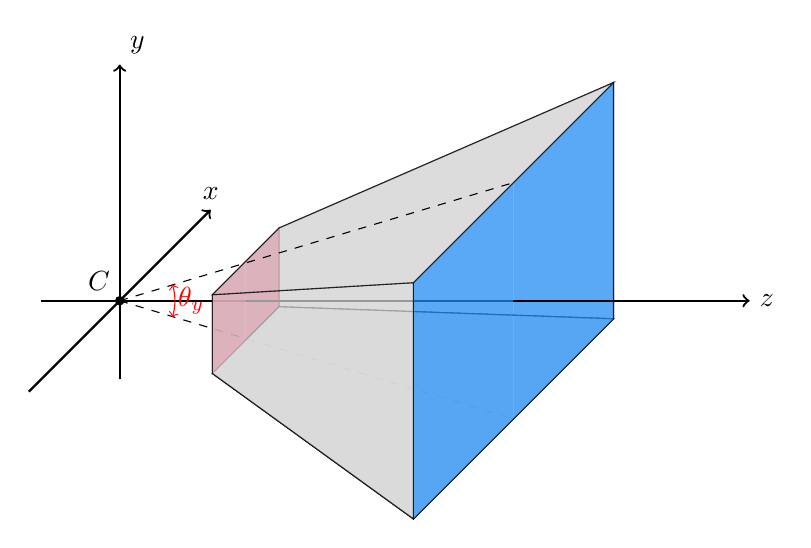
\begin{tikzpicture}[]
	
	%axes
	\def\Zmax{8}
	\def\Zmin{-1}
	\def\Ymax{3}
	\def\Ymin{-1}
	\def\Xmax{3}
	\def\Xmin{-3}

	%(Z,Y,X)
	\def\nearZ{1.6}
	\def\nearXmax{1.1}
	\def\nearYmax{0.5}

	\def\farZ{5}
	\def\farXmax{\nearXmax*3}
	\def\farYmax{\nearYmax*3}

	\coordinate (nearBotLeft)  at (\nearZ, -\nearYmax, -\nearXmax);
	\coordinate (nearTopLeft)  at (\nearZ,  \nearYmax, -\nearXmax);
	\coordinate (nearTopMid)  at (\nearZ, \nearYmax,  0);
	\coordinate (nearBotMid)  at (\nearZ, -\nearYmax, 0);
	\coordinate (nearTopRight) at (\nearZ,  \nearYmax,  \nearXmax);
	\coordinate (nearBotRight) at (\nearZ, -\nearYmax,  \nearXmax);
	\coordinate (farBotLeft)   at (\farZ, -\farYmax, -\farXmax);
	\coordinate (farTopLeft)   at (\farZ,  \farYmax, -\farXmax);
	\coordinate (farTopMid)  at (\farZ, \farYmax,  0);
	\coordinate (farBotMid)  at (\farZ, -\farYmax, 0);
	\coordinate (farTopRight)  at (\farZ,  \farYmax,  \farXmax);
	
	\coordinate (farBotRight)  at (\farZ, -\farYmax,  \farXmax);

	\definecolor{farplane}{HTML}{1E90FF}   % Dodger Blue (bright but not neon)
	\definecolor{nearplane}{HTML}{DC143C}    % Crimson Red (vivid but deep)

	%view frustum

	% fovy bottom line
	\draw[dashed] (0,0,0) -- (farBotMid);

	% near plane border
	\draw[black]
		(nearBotLeft) -- (nearTopLeft) -- (nearTopRight) -- (nearBotRight) -- cycle;

	% near plane (left side)
	\fill[fill=nearplane,opacity=0.7]
		(nearBotLeft) -- (nearTopLeft) -- (nearTopMid) -- (nearBotMid) -- cycle;
		
	% left plane
	\filldraw[fill=gray!30, draw=black, opacity=0.7]
		(nearBotLeft) -- (nearTopLeft) -- (farTopLeft) -- (farBotLeft) -- cycle;
	
	% bottom plane
	\filldraw[fill=gray!30, draw=black, opacity=0.7]
		(nearBotLeft) -- (nearBotRight) -- (farBotRight) -- (farBotLeft) -- cycle;

	% bottom plane
	\filldraw[fill=gray!30, draw=black, opacity=0.7]
		(nearBotLeft) -- (nearBotRight) -- (farBotRight) -- (farBotLeft) -- cycle;
	
	% far plane border
	\draw[black]
		(farBotLeft) -- (farTopLeft) -- (farTopRight) -- (farBotRight) -- cycle;

	% far plane (%left half)
	\fill[fill=farplane, opacity=0.7]
		(farBotLeft) -- (farTopLeft) -- (farTopMid) -- (farBotMid) -- cycle;
	%z axis
	\draw[->, thick] (\Zmin,0,0) -- (\Zmax,0,0) node[right] {$z$};

	% near plane (right side)
	\fill[fill=nearplane,opacity=0.7]
		(nearBotMid) -- (nearTopMid) -- (nearTopRight) -- (nearBotRight) -- cycle;

	% far plane (right half)
	\fill[fill=farplane, opacity=0.7]
		(farTopMid) -- (farTopRight) -- (farBotRight) -- (farBotMid) -- cycle;

	% right plane
	\filldraw[fill=gray!30, draw=black, opacity=0.7]
		(nearBotRight) -- (nearTopRight) -- (farTopRight) -- (farBotRight) -- cycle;
	
	% top plane
	\filldraw[fill=gray!30, draw=black, opacity=0.7]
		(nearTopLeft) -- (nearTopRight) -- (farTopRight) -- (farTopLeft) -- cycle;

	%fovy top line
	\draw[dashed] (0,0,0) -- (\farZ, \farYmax, 0);

	\draw[->, thick] (0,\Ymin,0) -- (0,\Ymax,0) node[above right] {$y$};
	\draw[->, thick] (0,0,-\Xmin) -- (0,0,-\Xmax) node[above] {$x$};

	% camera label
	\filldraw (0,0,0) circle[radius=1.5pt] node[above left] {$C$};

	\coordinate (origin) at (0,0,0);

	%fovy label
	\pic["\textcolor{red}{$\theta_y$}", draw=red, <->, angle eccentricity=1.3, angle radius=0.7cm]
		{angle=nearBotMid--origin--nearTopMid};

\end{tikzpicture}


	}
\end{figure}

\subsubsection{Deriving the Projection Matrix}
\begin{itemize}
	\item In this section we derive the Projection Matrix which maps the View Frustum to homogeneous Clip Space.
	\item We break it up into four steps
	\begin{enumerate}
		\item Scale $x$ and $y$ components such that perspective is captured.
		\item Scale $x$ and $y$ components again to $[-1,1]$ range
		\item Map $z$ to $[0,1]$ range such that relative depth is preserved
		\item Store original view space depth in $w$ variable
	\end{enumerate}

\end{itemize}
\textbf{1. Scale $x$ and $y$ such that perspective is captured}
\begin{itemize}
	\item To capture perspective, we project each vertex $v$ on the near plane via a line that passes through the origin and $v$.
	\item To project a vertex $\textbf{v}$ onto the near plane, we draw a line from the origin to that point and mark where it intersects the near plane.
	\item The parametric vector representing a line passing through points $A$ and $B$ is given by 
\[
	\textbf{r}(t) = \textbf{A} + t(\textbf{B} - \textbf{A}), t \in \mathbb{R}
\]

		In our case, $\textbf{A} = (0,0,0)$ and $\textbf{B}$ = $\textbf{v}$. Thus,

\[
	\textbf{r}(t) = \textbf{v}t
\]

We know that the $z$-component of the intersection point is going to be $n$.
\[
	\textbf{r}(t_i}) = (v_xt_i, v_yt_i, v_zt_i) \\
		         = (v_xt_i, v_yt_i, n)
\]

Equating the $z$-components: 
		\[
			t_i = n/v_z
		\]
Thus,
\[
	\textbf{r}(t_{i}) = \left(\frac{nv_x}{v_z}, \frac{nv_y}{v_z}, n\right)
\]

\item In other words, the projected $x$ and $y$ values of the vertex $\textbf{v}$ on the near plane will be ${nv_x}/{v_z}$ and ${nv_y}/{v_z}$ respectively. 

\begin{figure}[h!]
	\centering%
	\textbf{View Space}\\[0.5em]%
	\begin{subfigure}{0.45\textwidth}
	\resizebox{\textwidth}{!}{%
		\begin{tikzpicture}

\definecolor{topplane}{HTML}{2E8B57}   % Sea Green (clear, calm)
\definecolor{bottomplane}{HTML}{A0522D} % Sienna (warm earthy brown)
\definecolor{nearplane}{HTML}{1E90FF}   % Dodger Blue (bright but not neon)
\definecolor{farplane}{HTML}{DC143C}    % Crimson Red (vivid but deep)

	% parameters
\def\t{0.4} % tan(fov/2)
	\def\n{2.0}       % near
	\def\f{6.5}       % far
	\def\Zmax{7}      % drawing extent
	\def\Ymax{3}

	% axes
	\draw[->] (-0.5,0) -- (\Zmax+0.5,0) node[right] {$z$};
\draw[->] (0,-\Ymax) -- (0,\Ymax)       node[above] {$y$};

% top/bottom (black)
	\draw[] plot[domain=0:\Zmax] (\x,  { \t*\x});
	\draw[] plot[domain=0:\Zmax] (\x, {- \t*\x});

%top (colored)
	\draw[topplane] plot[domain=\n:\f] (\x,  { \t*\x});

%bottom (colored)
	\draw[bottomplane] plot[domain=\n:\f] (\x,  { -\t*\x});

% near/far from z = n, z = f  (verticals)
	% use the y-extent implied by the frustum at those z
	\draw[thick,nearplane, name path=near] plot[domain={- \t*\n}:{ \t*\n}] ({\n}, \x);
	\draw[thick,farplane, name path=far ] plot[domain={- \t*\f}:{ \t*\f}] ({\f}, \x);

	%extend near and far planes to inifinite with colored dotted lines
	\draw[dashed,nearplane, name path=near] plot[domain={-\Ymax}:{ \Ymax}] ({\n}, \x);
	\draw[dashed, farplane, name path=far ] plot[domain={- \Ymax}:{ \Ymax}] ({\f}, \x);

	% near / far labels
	\draw (\n, 0) node[below right] {$n$};
\draw (\f, 0) node[below right] {$f$};

% sample vertex
\def\vx{3.1}
\def\vy{0.9}
\draw[fill=black] (\vx,\vy) circle (1pt) node[above right] {$v_1$};

\def\ux{5.6}
\def\uy{0.9}
\draw[fill=black] (\ux,\uy) circle (1pt) node[above right] {$v_2$};

%label the origin as C, the Camera
\draw circle (0,0) node[below left] {$C$};

% line from origin to vertex
\draw[dashed, name path=vline] (0,0) -- (\vx,\vy);
\draw[dashed, name path=uline] (0,0) -- (\ux,\uy);

%label intersection between near plane and vline
\path[name intersections={of=vline and near, by=I}];
\path[name intersections={of=uline and near, by=IU}];
\fill (I) circle (1pt) node[above right];
\fill (IU) circle (1pt) node[below right];

%charmander graphic
\node at (3.3,0.45) {\includegraphics[height=1.2cm]{charmander_left_alpha.png}};
\node at (5.8,0.45) {\includegraphics[height=1.2cm]{charmander_left_alpha.png}};

%projection labels
\node (A) at (1,1) {$v_2'$};
\node (B) at (1,2) {$v_1'$};

% arrows from labels to points
\draw[->, bend right] (A) to (IU);
\draw[->, bend right] (B) to (I);
\end{tikzpicture}


	}
	\label{fig:2d-frustum-yz}
	\end{subfigure}%
\hfill
	\begin{subfigure}{0.45\textwidth}
	\resizebox{\textwidth}{!}{%
		\input{frustum-top.tikz}
	}
	\label{fig:2d-frustum-xz}
	\end{subfigure}

\caption{Side by side graps of the x-z slice and y-z slice of the view frustum showing the how the projected image is calculated on the near plane}
\end{figure}

\end{itemize}
\textbf{2. Scale $x$ and $y$ to $[-1,1]$ range}
\begin{itemize}
	\item Now, we just need to make sure that points inside the view frustum are mapped to normalized device coordinates. That is, points that intersect the top plane are mapped to y = 1, bottom y = -1, left x = -1, right x = 1.

	\item To do this, let the distance from the z axis to the top of the viewport be r and the distance from the z axis to right side of the viewport be r.

	\item To match the dimensions of our window, we define the aspect ratioo $a$ to be $a = r/t$

	\item We can calculate r by considering FIGURE X. $tan(\frac{\theta_u}{2}) = \frac{r}{n}$ so then $r = ntan(\frac{\theta_y}{2})$. 

	\item Then since $a = r/t$, $t = r/a$ which means $t = \frac{ntan(\frac{\theta_y}{2}}{a}$

	\item Now, if we scale the y component of all vertices on the near plane by $1/t$, this means that vertices in the range $[-r,r]$ will map to $[-1,1]$ and if we scale all the x components by $1/r$ all of the Vertices' x components will be in the range $[-1,1]$ which is exa tly what we need.
\begin{figure}[h!]
	\centering
	\textbf{View Space}\\[0.5em]%
	\resizebox{0.5\textwidth}{!}{%
		\begin{tikzpicture}
	\def\Xmax{3}
	\def\Ymax{3}

	% Viewport Box
	\def\botLeftX{-2.5}
	\def\botLeftY{-1.5}
	\def\topRightX{2.5}
	\def\topRightY{1.5}

	\filldraw[fill=red!20, draw=black]
    		(\botLeftX,\botLeftY) rectangle (\topRightX,\topRightY);

	% axes
	\draw[->] (-\Xmax,0) -- (\Xmax,0) node[right] {$x$};
	\draw[->] (0,-\Ymax) -- (0,\Ymax) node[above] {$y$};

	\def\smallGap{0.05}

	% r label
	\draw[decorate, decoration={brace, amplitude=6pt}, blue]
        	(\smallGap,\topRightY + \smallGap) -- (\topRightX - \smallGap,\topRightY + \smallGap)
        	node[midway, above=7pt, blue] {$r$};

	% t label
	\draw[decorate, decoration={brace, amplitude=6pt, raise=2pt}, red]
        	(\topRightX, \topRightY - \smallGap) -- (\topRightX,0+\smallGap)
        	node[midway, right=7pt, red] {$t$};

	%charmander graphic
	\node at (-0.6,0.35) {\includegraphics[height=1.8cm]{charmander_front_alpha.png}};
	\node at (0.4,0.36) {\includegraphics[height=1cm]{charmander_front_alpha.png}};

	\end{tikzpicture}


	}
	\caption{The view frustum from the perspective of the Camera}
	\label{fig:frustum-front}
\end{figure}

	
\item We now have what we need to figure out the firs two rows of the projection matrix. We need to scale the $x$ component by \textbf{TODO} and the $y$ component by \textbf{TODO} which can be done with the following matrix:
\[
\mathbf{Pv} =
\begin{pmatrix}
m_{11} & m_{12} & m_{13} & m_{14} \\
m_{21} & m_{22} & m_{23} & m_{24} \\
m_{31} & m_{32} & m_{33} & m_{34} \\
m_{41} & m_{42} & m_{43} & m_{44}
\end{pmatrix}%
\begin{pmatrix}
x \\ y \\ z \\ 1
\end{pmatrix}
=
\begin{pmatrix}
x\\y\\z\\1
\end{pmatrix}
\]

\end{itemize}
\textbf{3. Scale $z$ to $[0,1]$ range}
\begin{itemize}
	\item In order to determine the matrix elements that will transform the input $v_z$ into the desired $[0,1]$ range, we work backwards by considering what elements would be needed to map a point on the near plane to $z = 0$ and a point on the far plane to $z = 1$
	\item  We would need
\[
\begin{pmatrix}
m_{11} & m_{12} & m_{13} & m_{14} \\
m_{21} & m_{22} & m_{23} & m_{24} \\
m_{31} & m_{32} & m_{33} & m_{34} \\
m_{41} & m_{42} & m_{43} & m_{44}
\end{pmatrix}%
\begin{pmatrix}
x \\ y \\ n \\ 1
\end{pmatrix}
=
\begin{pmatrix}
x\\y\\0\\1
\end{pmatrix}
\]

\[
\begin{pmatrix}
m_{11} & m_{12} & m_{13} & m_{14} \\
m_{21} & m_{22} & m_{23} & m_{24} \\
m_{31} & m_{32} & m_{33} & m_{34} \\
m_{41} & m_{42} & m_{43} & m_{44}
\end{pmatrix}%
\begin{pmatrix}
x \\ y \\ f \\ 1
\end{pmatrix}
=
\begin{pmatrix}
x\\y\\1\\1
\end{pmatrix}
\]

\item We would need $m_{33}$ and $m_{34}$ to be \textbf{TODO} and \textbf{TODO} respectively

\item How we do this mapping doesn't actually matter that much, as long as relative ordering is preserved. 
\end{itemize}
\textbf{4. Store $w$ value}
\begin{itemize}
	\item Simply set $m_{43}$ to be 1
	\item Talk about homogeneous coordinates
\end{itemize}
\textbf{The Final Matrix}
\begin{itemize}
	\item Combining all the steps together, the final matrix is given by:

\[
	\textbf{P} = 	
\begin{pmatrix}
m_{11} & m_{12} & m_{13} & m_{14} \\
m_{21} & m_{22} & m_{23} & m_{24} \\
m_{31} & m_{32} & m_{33} & m_{34} \\
m_{41} & m_{42} & m_{43} & m_{44}
\end{pmatrix}%
\begin{pmatrix}
x \\ y \\ z \\ 1
\end{pmatrix}
=
\begin{pmatrix}
x\\y\\z\\w
\end{pmatrix}
\]
\end{itemize}

\subsubsection{Perspective Divide}
\begin{itemize}
	\item Once we have applied the perspective 
\end{itemize}
\subsection{Deriving The Viewport Matrix}
\subsection{Clipping \& The Sutherland Hodgman Algorithm}

\section{Drawing to the screen}
\subsection{What is \textit{Rasterization}?}
\subsection{Interpolation}
\subsection{Rasterizing Triangles}
\subsection{What is a \textit{Fragment?}}
\subsection{The Fragment Shader}
\subsection{Depth Testing}
\subsection{The Framebuffer and Z-Buffer}

\section{Shading}

\subsection{Shaders}
\subsection{Materials}
\begin{itemize}
	\item A Material
	\item It contains ...
\end{itemize}

\subsection{Textures}
\subsection{Unlit Shader}
\subsection{Lit Shader}
\subsection{Phong Shader}
\subsection{Toon Shader}
\subsection{Shadows}
\subsection{Ambient Occlusion}

\section{Appendix}
\subsection{Quaternions}
\subsection{Barycentric Coordinates}
\section{Deprecated}
\subsection{Math Concepts}
\subsubsection{Vectors}
\begin{itemize}
\item In this document, we will use typical Vector operations and notation including but not limited to the following
\item A vector is $\textbf{v}$ is a collection of real numbers denoted by 
\item The \textit{dot product} is defined by
\item The \textit{cross product} is defined by
\item A unit vector is denoted by the hat
\end{itemize}

\subsubsection{Planes}
\begin{itemize}
	\item A plane is defined by \textbf{**TODO**}
\end{itemize}
\subsubsection{Matrices}

\begin{itemize}
	\item To understand Graphics Engines, you must become somewhat familiar with the operation of matrices. In particular: Matrix Multiplication, Inverse Matrices, Matrices as Linear Transformations and probably more. I provide a very scarce review below.
	\item Matrix multiplication is done like so:
	\item Matrix Inverse is calculated like so:
	\item For an affine, orthonormal matrix, the inverse can be calculated like this ( + reference)
\end{itemize}
\subsubsection{Quaternions}
\begin{itemize}
	\item To represents rotations in 3D space, I use Quaternions. While you can use a composition of 3x3 Euler Matrices, they are slower, hard to interpolate and are at risk of Gimbal Lock (+ Reference).
	\item A Quaternion is a kind of 4D complex number $q = q_0 + q$ where $q_0$ is a scalar and
$q$ is an R3 vector where each component has unit vectors $i, j, k$.
	\item The unit vectors $i,j,k$ adhere to the following multiplication rules. \textbf{**TODO**}
	\item Whenever you are interested in rotating an object in 3D space, you need to specify 2 things: An axis and an angle. These are encoded in the Unit Quaternion in the following way: \textbf{**TODO**}
	\item In the space of Unit Quaternions, if you operate a Unit Quaternion on a Vector, it results in a rotation of some degrees about some axis.
\end{itemize}
\subsubsection{Coordinate Spaces}
\begin{itemize}
	\item Cartesian
	\item Projective
	\item Barycentric
	\item Spherical, Cylindrical
\end{itemize}
\subsubsection{Transformations}
\begin{itemize}
	\item Model, View, Projection
\end{itemize}
\subsubsection{Deriving the Model Matrix}
\subsubsection{Deriving the View Matrix}
\subsubsection{Deriving the Projection Matrix}

The Projection Matrix is responsible for converting vertices from View space into Clip space. It aims to morph points that lie inside or on the View frustum into the Canonical View Volume in such a way that \textit{perspective} is introduced.  

\par\medskip
Perspective is described simply by the idea that things that are far away seem small and things that are close seem big.

\par\medskip
We break the problem  up into 2 parts:
\begin{enumerate}
	\item Calculating the transformation for $x$ and $y$
	\item Calculating the transformation for $z$
\end{enumerate}

For the first part, consider the setup in Figure ?. In this 2D slice, the viewing volume is given by the near and far planes and the top and bottom planes. What we wish to do is to take some point $v$, and project it onto the near plane. 

To do this, we draw a line from the point to the origin. Consider the point at which this origin ray intersects the near plane. Let's call this point $x$. 

\subsubsection{Deriving the Viewport Matrix}
\subsection{Algorithms}
\subsubsection{Rasterization}
\subsubsection{Improved Rasterization}
\begin{itemize}
	\item (First Approach) Takes a Primitive (Triangle made of Vertices) after is has been transformed by MVP and VP. It computes Bounding Box and using BaryCentric Coordinates with respect to the Triangle vertex positions decides which pixels to remove based on whether they are inside or outside of the triangle \textbf{**FIGURE**}
	\item (Optimized Approach) Iterative Edge Functions \textbf{**TODO**}
\end{itemize}

\subsubsection{Clipping}
\begin{itemize}
	\item After the Vertex Shader is applied, triangle vertices should be in \textit{Clip Space}, which is a \textit{homogeneous vector space} in $R^4$ where $v = (x,y,z,w)$ maps to $u = (x/w, y/w, z/w)$ in $R^3$
	\item The goal of this algorithm is to \textit{clip} the triangle against the \textit{View Frustum}, which in homoegenous space is a volume bounded by 6 4D planes.
	\item We start by deriving an expression for each planes, represented by a normal vector $n \in \mathbb{R}^4$ and some point on the vector $p \in \mathbb{R}^4$
	\item The projection matrix maps each of the 6 $\mathbb{R}^3$ planes that define the view frustum. \textbf{**TODO**} Show that the 6 view frustum planes map to the planes used in 4 space

\item \textbf{**TODO**} Write some pseudocode, include a diagram

\end{itemize}
\section{Conclusion \& Future Work}

\subsection{What I learnt}

\subsection{Limitations}

\subsection{A future implementation in C++}


\section{References}

\end{document}

